%% OTA-Shield : IJCIP submission (Elsevier cas-dc, single-blind, numbered refs).
\documentclass[a4paper,fleqn]{cas-dc}

\usepackage{lmodern}
\usepackage[T1]{fontenc}
\usepackage[utf8]{inputenc}
\usepackage{microtype}
\usepackage[numbers,sort&compress]{natbib}
\usepackage{amsmath,amssymb}
\usepackage{booktabs}
\usepackage{graphicx}
%% Figures live in figures/.
\graphicspath{{figures/}}
\usepackage{xcolor}
\usepackage{hyperref}
\hypersetup{breaklinks=true,
            pdfauthor={},
            pdftitle={OTA-Shield: A Hardware-Measured Reference Architecture for In-Network OTA Rollout Admission and Bounded Firmware-Attack Detection in Battery Energy Storage Systems},
            pdfsubject={},
            pdfkeywords={}}
\usepackage{xurl}           % aggressive URL line-breaking in bibliography
\usepackage{algorithm}
\usepackage{algpseudocode}
\usepackage{tikz}
\usetikzlibrary{arrows.meta, positioning, fit, backgrounds,
                 shapes.geometric, calc}
\usepackage{pgfplots}
\pgfplotsset{compat=1.16}
\usepackage{float}
\usepackage{placeins}       % provides \FloatBarrier
\usepackage{listings}

\lstset{basicstyle=\footnotesize\ttfamily, breaklines=true}

%% Auto-generated numeric macros : never hardcode a result number.
\InputIfFileExists{numbers.tex}{}{%
  \PackageWarning{OTA-Shield}{numbers.tex not found}}
\InputIfFileExists{numbers_e12b_signed_inotify_full.tex}{}{%
  \PackageWarning{OTA-Shield}{numbers_e12b_signed_inotify_full.tex not found}}
\InputIfFileExists{numbers_supplement.tex}{}{%
  \PackageWarning{OTA-Shield}{numbers_supplement.tex not found}}

%% Convenience
\newcommand{\otashield}{OTA-Shield}
\newcommand{\tofino}{Tofino~1}
% RV-2: clean prime for the stochastic-rollback experiment name (was \Enineteenp{},
% which rendered/extracted as "E190"). Text superscript prime renders cleanly.
\newcommand{\Enineteenp}{\texorpdfstring{E19\textsuperscript{\textquotesingle}}{E19'}}

\usepackage{xr-hyper}
\externaldocument{main}
\begin{document}
\renewcommand{\thesection}{S\arabic{section}}
\renewcommand{\thetable}{S\arabic{table}}
\renewcommand{\thefigure}{S\arabic{figure}}
\renewcommand{\theequation}{S\arabic{equation}}
\setcounter{section}{0}\setcounter{table}{0}\setcounter{figure}{0}

\shorttitle{Supplementary material: \otashield}
\shortauthors{Akekudaga et~al.}
\title[mode=title]{Supplementary Material: \otashield{}}
\author[1]{Philip Akekudaga}
%% TODO: provide Simon's affiliation.
\author[2]{Simon Wewoliamo Kuseh}
\author[3]{Mubarak Hussein}
\affiliation[1]{organization={University of Rhode Island}, city={Kingston}, state={RI}, country={USA}}
\affiliation[2]{organization={Affiliation to be provided}}
\affiliation[3]{organization={University at Albany, SUNY}, city={Albany}, state={NY}, country={USA}}
\begin{abstract}
This document provides supplementary figures, tables, and methodological detail supporting the main paper: per-trial results, the first-contact recall taxonomy, build provenance, the statistical methodology, per-component resource placement, and the boundary and capacity floats referenced from the evaluation.
\end{abstract}
\begin{keywords}
Supplementary material
\end{keywords}
\maketitle

\section{Build provenance and the R5-gating revision}\label{app:build-provenance}

The results in this paper were collected on two successive binaries, and
this appendix records which experiment ran on which so that each number can
be tied to a fixed configuration. The deployed build gates the fleet-fanout
counter (R5) on the unauthorized-source flag (\texttt{r2\_fired}) and arms
the per-source \texttt{hold\_armed\_reg} gate only on R5; because R5 sits
behind the terminal R2 drop, that gate is inert on reachable input
(\S\ref{sec:cascade-fix}, \S\ref{sec:known-correctness}). An earlier
un-gated build armed the per-source gate on \emph{any} rule fire. On that
build a compressed benign rollout that tripped the per-BMS replay rule (R1)
would arm the gate and drop the source's subsequent packets at line rate
before the arbiter could clear them, producing benign-rollout false
positives. Restricting the gate's arming to R5 removes this behavior, and
E12, E19, and \Enineteenp{} were re-measured on the deployed build, where
they report zero benign-rollout false positives (\S\ref{sec:e12},
\S\ref{sec:e19p}).

One consequence of the revision is the rollback recall the deployed build
reports. The un-gated build recorded a near-perfect rollback recall, but
that figure was inflated: the per-source gate incidentally dropped
first-contact rollbacks that R6 itself cannot catch, because a first
contact to a BMS has no stored version high-water mark. On the deployed
build those cold-start cases surface as the gap between strict
recall (\EOneNineprollbackstochasticRecallMean{}, counting first-contact
events as misses) and lenient recall
(\EOneNineprollbackstochasticRecallLenientMean{}); we report the strict
figure (\S\ref{sec:e19p}, Appendix~\ref{app:e19p-firstcontact}).

The five-state lifecycle matrix (E22, \S\ref{sec:e22}) was originally
completed only on the un-gated binary, where the per-source gate pre-empts
the arbiter (152 of 160 benign rollout events dropped, a 95\%
false-positive rate). We re-ran the in-scope active-authorized state on the
deployed gated build (0 false positives across 80 events, confirming the
fix); the remaining states probe off-parameter authorized operation that
the gated build does not quarantine (\S\ref{sec:e22}), and a
containment matrix that also exercises a per-source hold role would require
the 5-tuple-indexed hold register of \S\ref{sec:known-correctness} behind a
P4 recompile. The integrity and freshness lifecycle failure modes are
covered by E12b (\S\ref{sec:e12b}). Table~\ref{tab:provenance} summarizes
the per-experiment configuration.

\begin{table*}[pos=htbp]
  \centering
  \caption{Per-experiment build provenance. ``Deployed gated'' is the final
  binary (R5 r2-gated, per-source hold gate inert, 5-tuple-keyed override
  table); ``un-gated'' is the earlier binary used before the R5-gating
  revision. The last column marks whether the result is part of the
  deployed-build story or is auxiliary/motivating only.}
  \label{tab:provenance}
  \footnotesize
  \begin{tabular}{@{}l l l c@{}}
    \toprule
    Experiment(s) & Binary & R5 gating & Deployed story \\
    \midrule
    E1, E2, E6, E8, E14      & deployed gated & r2-gated & yes \\
    E4 (arbiter ablation)    & deployed gated & r2-gated & yes \\
    E12, E12b                & deployed gated & r2-gated & yes \\
    E19, \Enineteenp{}       & deployed gated & r2-gated & yes \\
    E9, E21, E23, E20        & deployed gated & r2-gated & yes \\
    E10 (incl.\ symmetric)   & deployed gated & r2-gated & yes \\
    E11, E13, E18            & deployed gated & r2-gated & yes \\
    E7b (long-horizon)       & deployed gated & r2-gated & yes \\
    \midrule
    S1, S2 (200-BMS)   & earlier binary & n/a      & scope only (cap-limited) \\
    E22 active-authorized    & deployed gated & r2-gated & yes (confirms fix) \\
    E22 full matrix          & un-gated       & ungated  & motivating only \\
    \bottomrule
  \end{tabular}
\end{table*}

\noindent The override table is 5-tuple-keyed on the deployed build
throughout (\S\ref{sec:e13}); E13 additionally characterizes the optional
source-IP aggregation variant. E7b was re-run on the deployed gated build
(\S\ref{sec:e7b}): over the 8~h trace it records 0 benign false positives
and catches all 100 rollback attacks, so it now reports on the deployed
binary rather than an un-gated auxiliary run.

\section{Supplementary figures and tables}\label{app:supp}

\begin{table*}[pos=htbp]
  \centering
  \caption{Rollout-Authorization Table fields. The manifest is a
  per-rollout JSON object loaded by the controller; a HOLD packet
  passes only when every condition matches.}
  \label{tab:rat}
  \footnotesize
  \begin{tabular}{@{}l p{0.70\textwidth}@{}}
    \toprule
    Field & Policy semantics \\
    \midrule
    \texttt{authorized\_source\_ips}  & Allow-list of IPv4 addresses
        permitted to originate firmware PUBLISHes for this rollout. \\
    \texttt{target\_bms\_list}        & Allow-list of destination BMS
        IPs within scope of the rollout. \\
    \texttt{valid\_window\_start/end} & UTC wall-clock window during
        which the rollout is active. \\
    \texttt{expected\_payload\_size\_range} & Inclusive byte range for
        advertised firmware size. \\
    \texttt{expected\_firmware\_version}    & Version number reported in
        the OTA header for control-plane sanity check. \\
    \texttt{max\_concurrent\_targets} & Enforced per-rollout cap on the
        number of concurrent active sessions a rollout may hold; the
        controller denies admission beyond it (0~$=$~unlimited). \\
    \texttt{rollback\_window}         & Optional
        \{\texttt{min\_version}, \texttt{max\_version}\} pair
        authorizing a rollback range for this rollout
        (see \S\ref{sec:rat-gates-6b}). Default-absent: R6 remains a
        terminal rule. \\
    \bottomrule
  \end{tabular}
\end{table*}

\begin{table}[pos=htbp]
  \centering
  \caption{Reference-channel parser portability (E18) across the
  \EeighteenMfourVariants{}-variant MQTT-parameter sweep on the deployed
  parser. PARSED = the parser extracted a valid OTA header; PARSER-MISS =
  the packet was classified as non-OTA and forwarded unflagged. No variant
  is dropped; the determining factor is the 32-byte topic slot, not QoS or
  the retain flag.}
  \label{tab:e18}
  \footnotesize
  \begin{tabular}{@{}l l l@{}}
    \toprule
    Variant & Parameters & Outcome \\
    \midrule
    baseline      & topic=32~B, QoS=1, retain=0 & PARSED \\
    QoS=2         & topic=32~B, QoS=2, retain=0 & PARSED \\
    retain=1      & topic=32~B, QoS=1, retain=1 & PARSED \\
    QoS=0         & topic=32~B, QoS=0, retain=0 & PARSED \\
    short topic   & topic=16~B, QoS=1, retain=0 & PARSER-MISS \\
    long topic    & topic=64~B, QoS=1, retain=0 & PARSER-MISS \\
    QoS=0, short  & topic=16~B, QoS=0, retain=0 & PARSER-MISS \\
    QoS=0, long   & topic=64~B, QoS=0, retain=0 & PARSER-MISS \\
    \bottomrule
  \end{tabular}
\end{table}

\begin{table}[pos=htbp]
  \centering
  \caption{50-BMS vs.\ 200-BMS precision and F\textsubscript{1}. Recall is
  1.000 across the 200-BMS replays (S1, S2); the 50-BMS E8 row reflects nine
  near-threshold R1 misses (recall \EEightstochasticRecallMean{}). No rollback
  attempt is missed at either scale. The
  precision collapse at 200-BMS is attributed to the 64-entry
  controller/manifest BMS cap. The data-plane \texttt{bms\_ip\_to\_idx}
  table is itself compiled at 128 entries (Table~\ref{tab:mau-resource}),
  so legitimate packets addressed to BMS~65--200 are unmapped and take the
  fail-closed DROP path.}
  \label{tab:fleet-scaling}
  \small
  \begin{tabular}{@{}l c c c c@{}}
    \toprule
    Experiment & Fleet & Precision & Recall & F\textsubscript{1} \\
    \midrule
    E8 (50-BMS headline)  & 50  & \EEightstochasticPrecisionMean{} & \EEightstochasticRecallMean{} & \EEightstochasticFOneMean{} \\
    S1 (200-BMS, det.)  & 200 & \EOnePrimePrecision{}           & \EOnePrimeRecall{}            & \EOnePrimeFOne{} \\
    S2 (200-BMS, stoch.) & 200 & \EEightPrimePrecision{}         & \EEightPrimeRecall{}          & \EEightPrimeFOne{} \\
    \bottomrule
  \end{tabular}
\end{table}

\begin{table*}[pos=htbp]
  \centering
  \caption{CPU IDS baselines on identical traffic (E10), on the E1 PCAP replay
  (\EtenSuricataNDecisions{}~events: 60 attack + 30 legitimate).
  Variants (i)--(iv) are CPU-IDS configurations; variants~(v) and~(vi)
  post-process variants~(i) and~(iii)'s alerts respectively through the
  same RAT arbiter \otashield{} uses in-band (the apples-to-apples
  controls).}
  \label{tab:e10variants}
  \footnotesize
  \begin{tabular}{@{}l c c c c c@{}}
    \toprule
    Variant & Prec. & Recall & Acc. & TP & FP \\
    \midrule
    (i) Suricata min-effort        & N/A                               & \EtenSuricataRecall            & \EtenSuricataAccuracy          & 0  & 0 \\
    (ii) Suricata stateful         & \EtenSuricataStatefulPrecision    & \EtenSuricataStatefulRecall    & \EtenSuricataStatefulAccuracy  & \EtenSuricataStatefulTP & \EtenSuricataStatefulFP \\
    (iii) Suricata permissive      & \EtenSuricataPermPrecision        & \EtenSuricataPermRecall        & \EtenSuricataPermAccuracy      & \EtenSuricataPermTP     & \EtenSuricataPermFP \\
    (iv) Zeek domain-aware         & \EtenZeekPrecision                & \EtenZeekRecall                & \EtenZeekAccuracy              & \EtenZeekTP             & \EtenZeekFP \\
    (v) Suricata + RAT             & N/A                               & \EtenSuricataRatRecall         & \EtenSuricataRatAccuracy       & \EtenSuricataRatTP      & \EtenSuricataRatFP \\
    (vi) Suricata permissive + RAT & \EtenSuricataPermRatPrecision     & \EtenSuricataPermRatRecall     & \EtenSuricataPermRatAccuracy   & \EtenSuricataPermRatTP  & \EtenSuricataPermRatFP \\
    \bottomrule
  \end{tabular}
\end{table*}

\begin{table*}[pos=htbp]
  \centering
  \caption{Defence-in-depth coverage. Each layer catches a different
  fraction of the attack space; \otashield{} is one of the three, not a
  replacement for the others.}
  \label{tab:layers}
  \footnotesize
  \begin{tabular}{@{}l p{0.70\columnwidth}@{}}
    \toprule
    Layer & What it catches \\
    \midrule
    Endpoint signing (SUIT/Uptane) & Unsigned or mis-signed firmware at
      the BMS, regardless of how it arrives. Blind to
      \emph{signed-but-malicious} firmware (stolen signing key) and blind
      to in-transit fanout. \\
    \otashield{} data plane    & Naive coordinated campaigns (A1--A4 at
      their designed thresholds, plus A5 rollback via R6 and Gate~B) at
      the network aggregation point. Blind to shaped adversaries that
      stay inside rule blind zones (E21); requires placement after
      TLS/VPN termination (\S\ref{sec:discussion}). \\
    Operator rollout dashboard & Slow-drift campaigns visible over hours
      to days through fleet-version skew. Too slow to stop a
      minutes-scale attack in flight. \\
    \bottomrule
  \end{tabular}
\end{table*}

\begin{figure}[pos=htbp]
  \centering
  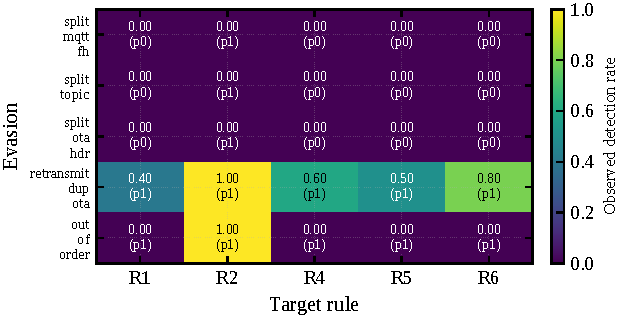
\includegraphics[width=0.92\columnwidth]{figures/F15_tcp_evasion.pdf}
  \caption{TCP-segmentation evasion (E23): observed per-cell drop
  rate over 10 trials/cell (250 trials), each cell reset-isolated; cell
  text is observed rate (predicted in parens). Header-split evasions
  defeat every rule including the source-keyed R2; only
  \texttt{retransmit-dup} (intact PUBLISH on the wire) yields
  parse-dependent detection, and only probabilistically. The R5 column
  does not exercise genuine fanout (single-PUBLISH base attack) and is
  shown for completeness.}
  \label{fig:tcp-evasion}
\end{figure}

\begin{figure}[pos=htbp]
  \centering
  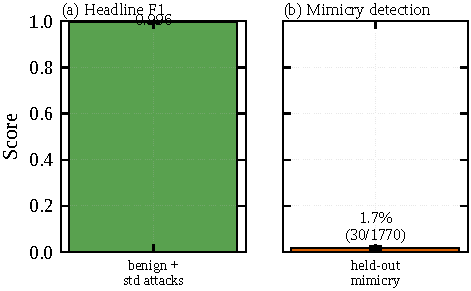
\includegraphics[width=0.92\columnwidth]{figures/F11_co_equal_headline.pdf}
  \caption{The two headline numbers, shown co-equal on a common
  $[0,1]$ scale: (a)~naive fleet-fanout detection
  F\textsubscript{1}~=~\EEightstochasticFOneMean{} (E8) versus
  (b)~adaptive-mimicry coverage \EOneSevenmimicryStrategyCatchPct\%
  (E21). The headline applies to the designed naive family; an adversary
  who reshapes cadence faces the right-hand number.}
  \label{fig:co-equal}
\end{figure}

\begin{table}[pos=htbp]
  \centering
  \caption{Rule fires per mimicry strategy (E21) under
  per-strategy isolation, summed over \EOneSevenmimicryNTrials{}
  campaigns (\EOneSevenmimicryStrategyTotal{} attack events total).
  Each strategy is designed to evade a specific data-plane rule;
  ``caught'' counts events the controller dropped, ``missed'' counts
  everything else. Under isolation, only \emph{R1-late} produces any
  drop; every sub-threshold strategy evades entirely. Missed events
  escape the data plane and would need control-plane or endpoint
  recovery.}
  \label{tab:mimicry}
  \footnotesize
  \begin{tabular}{@{}l r r r r r r r@{}}
    \toprule
    Strategy & N & R1 & R2 & R4 & R5 & caught & missed \\
    \midrule
    fanout-sub    & 720 &  0 &  0 &  0 &  0 &  0 & 720 \\
    fanout-three  & 540 &  0 &  0 &  0 &  0 &  0 & 540 \\
    R4-deadzone   &  90 &  0 &  0 &  0 &  0 &  0 &  90 \\
    combined      & 360 &  0 &  0 &  0 &  0 &  0 & 360 \\
    R1-late       &  60 & 30 &  0 &  0 &  0 & 30 &  30 \\
    \midrule
    Total         &\EOneSevenmimicryStrategyTotal{}& 30 & 0 & 0 & 0
                  &\EOneSevenmimicryStrategyCaught{}
                  &\EOneSevenmimicryStrategyMissed{} \\
    \bottomrule
  \end{tabular}
\end{table}

\begin{table*}[pos=htbp]
  \centering
  \caption{Tofino resource footprint of the evaluated build, with rough
  comparison to a CPU-based alternative on the same traffic.
  Dollar-per-BMS-year assumes a five-year amortization of a USD~20\,k
  switch over a 50-unit fleet.}
  \label{tab:cost}
  \footnotesize
  \begin{tabular}{@{}l l l@{}}
    \toprule
    Cost dimension & \otashield{} (\tofino{}) & Suricata (Xeon Gold) \\
    \midrule
    MAU stages used              & 12 of 12 (Table~\ref{tab:mau-resource}) & n/a \\
    SRAM for rule state          & 3\,KB (R5 Bloom) + 0.5\,KB (R1) & host RAM \\
    Session table (fleet-wide)   & 512\,KB (two 64\,K $\times$ 32\,bit) & host RAM \\
    Power per Gb/s (amortized)   & $\sim$70\,mW/Gb/s         & $\sim$5\,W/Gb/s \\
    Throughput headroom          & measured 2{,}200\,pps (generator-bound); ASIC 25\,Gb/s link, unmeasured & 40--60\,Gb/s~\cite{hu2019analysinghighspeed} \\
    Hardware cost (list)         & \$20\,k (32$\times$100\,GbE) & \$8--12\,k server \\
    \$/BMS-year (50-unit fleet)  & $\approx$\$80             & $\approx$\$40 \\
    \bottomrule
  \end{tabular}
\end{table*}

{\footnotesize
\setlength{\bibsep}{1pt plus 0.2ex}
\bibliographystyle{unsrtnat}

{\footnotesize
\setlength{\bibsep}{1pt plus 0.2ex}
\bibliographystyle{unsrtnat}
\bibliography{references}
}
\end{document}
